\section{Гомогенное преобразование. Тензор положения. Тензор скорости.}\label{geom}

Остановимся подробнее на введенном в рассмотрение объекте гомогенного преобразования, математическое представление которого может быть различным. В частности, для него могут применяться матрицы размерностью 4x4, бикватернионы, комбинация кватерниона поворота и вектора трансляции и т.д. В рамках рассматриваемого метода конкретная форма представления объекта взаимозаменяема и определяется исключительно удобством реализации в вычислительной системе. Обозначим объект гомогенного преобразования и тензор преобразования, выполняемого объектом как $H^j_i$. 

В програмной реализации удобно представлять $H^j_i$ как комбинацию двух компонент, кватерниона поворота $Q$ и вектора трансляции $S$, но, как сказано ранее есть и иные возможные представления. 

На множестве $H^j_i$ определена операция некомутативная операция композиции, часто обозначаемая как умножение. Множество $H^j_i$ замкнуто по этой операции.

Введем в рассмотрение объект положения СК и связанный с ним тензор положения. Обозначим его P. Объект положения удобно задавать тем же набором компонент, что и объект гомогенного преобразования. В такой нотации компонентное выражение тензора положения $P$ j-ой системы координат взятого в i-том базисе, будет совпадать с компонентным выражением тензора преобразования СК, из базиза i-той СК в базис связанный с j-ой СК. 

\begin{equation}
P_j^{(i)} = H_{ij}^{(i)}
\end{equation}

Также введем в рассмотрение производную тензора положения j-ой системы координат

\begin{equation}\label{speed_eq} 
V_j(t) = P_j'(t) 
\end{equation}

Как и тензор преобразования системы координат и тензор положения, производная тензора положения является геометрическим объектом и имеет смысл скорости изменения геометрического положения объекта или системы координат. Часто в качестве компонентного представления производной тензора представления выбирают производные компонент тензора положения, однако такой подход не является интуитивным и не очень удобен в вычислительной реализации. В настоящем методе в качестве компонентного представления производной тензора положения выбирается пара векторов его линейной и угловой скорости $(v,\omega)$

\begin{equation}\label{speed_eq_comp} 
V_j(t) = \dot{P}_j(t) = (\omega_j(t),v_j(t)) 
\end{equation}

При необходимости, корректность такого перехода может быть выведена аналитически в нотации бикватерионов. 

Представление (\ref{speed_eq}), удобно, в рамках метода, с вычислительной точки зрения. Следует учесть, что использование такой системы компонентного представления приводит к тому, что уравнение (\ref{speed_eq}) не может быть в общем случае записано в компонентной форме.

\colorbox{shadecolor}
{\parbox{0.9\textwidth}{Вектор, состоящий из компонент пары векторов $(\omega, v)$ далее называется 6-вектором скорости кинематического звена. Альтернативное представление тензора положения в виде пары радиус вектора и вектора поворота $(r,\rho)$ далее называется 6-вектором положения.}}

Одной из возможных форм компонентного представления тензора положения является пара радиус-вектора и вектора поворота $(r,\rho)$ (порядок преобразований - сначала поворот, затем трансляция). Отметим, что, если на 6-вектор скорости $(v,\omega)$ наложить условие колинеарности 6-вектору положения $(r,\rho)$, задача может быть сведена к одномерной, дифференциальные уравнения становятся линейными, а композиции преобразований по этой 6-оси становятся комутативными и образуют группу. 
\begin{center}
  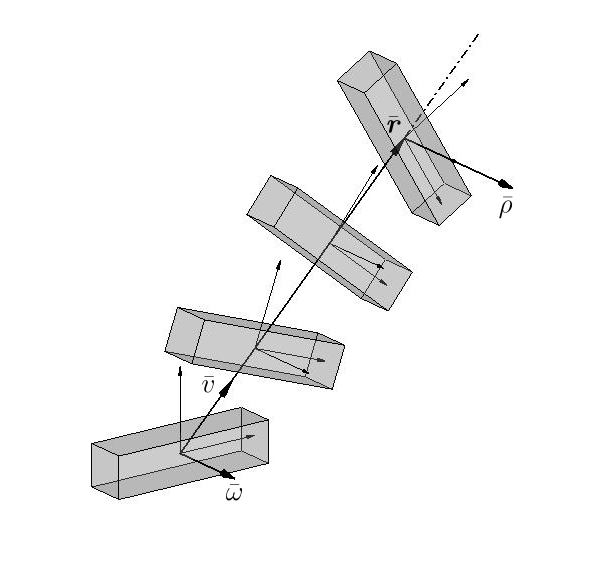
\includegraphics[width=0.8\textwidth,height=0.8\textheight,keepaspectratio]{oneaxis.png}
  \captionof{figure}{Сведение задачи к одномерному случаю.}
  \label{}
\end{center}

В форме 3-векторов для этого должны выполняться соотношения.
\begin{equation}\label{} 
\bar{v} \upuparrows \bar{r}, \  \bar{\omega} \upuparrows \bar{\rho}, \  \frac{|\bar{v}|}{|\bar{r}|} = \frac{|\bar{\omega}|}{|\bar{\rho}|} 
\end{equation}
\begin{equation}
(\bar{v_l},\bar{\omega_l}) = (\dot{\bar{r_l}},\dot{\bar{\rho_l}})
\end{equation}

Это замечание пригодится для дальнейшего изложения и может быть полезно при анализе устойчивости системы управления в терминах объектов гомогенных преобразований. 

Хочется отметить, что анализ устойчивости систем управления в терминах алгебраических объектов, отличных от действительных чисел, таких как объекты гомогенных трансформаций может иметь существенное практическое значение и представляет интересное направление исследований.